\subsection{Magnetfelder verschiedener Spulen}
Es wird an zwei unterschiedlich langen Spulen die magnetische Flußdichte vermessen.

\subsubsection{Lange Spule}
Die Messwerte für die lange Spule werden in der Tabelle \ref{tab:ls} aufgeführt und sind in der Abbildung \ref{fig:ls} zu betrachten.
Der Ursprung in der Grafik liegt auf dem Anfangspunkt der Spule.
Die Mitte der Spule liegt bei $x=\SI{0.09}{m}$.
\documentclass[captions=tableheading]{scrartcl}
\usepackage{booktabs}
\usepackage{pdflscape}




\begin{document}
%\begin{landscape}


\begin{table}
  \centering
  \caption{Messdaten}
  \label{tab:some_data}
  \begin{tabular}{c c }
    \toprule
     x &	 B	   \\
     cm &   mT  \\
    \midrule
      \documentclass[captions=tableheading]{scrartcl}
\usepackage{booktabs}
\usepackage{pdflscape}




\begin{document}
%\begin{landscape}


\begin{table}
  \centering
  \caption{Messdaten}
  \label{tab:some_data}
  \begin{tabular}{c c }
    \toprule
     x &	 B	   \\
     cm &   mT  \\
    \midrule
      \documentclass[captions=tableheading]{scrartcl}
\usepackage{booktabs}
\usepackage{pdflscape}




\begin{document}
%\begin{landscape}


\begin{table}
  \centering
  \caption{Messdaten}
  \label{tab:some_data}
  \begin{tabular}{c c }
    \toprule
     x &	 B	   \\
     cm &   mT  \\
    \midrule
      \input{Langsp.txt}
    \bottomrule
  \end{tabular}
\end{table}

%\end{landscape}
\end{document}

    \bottomrule
  \end{tabular}
\end{table}

%\end{landscape}
\end{document}

    \bottomrule
  \end{tabular}
\end{table}

%\end{landscape}
\end{document}

\begin{figure}[h!]
  \centering
  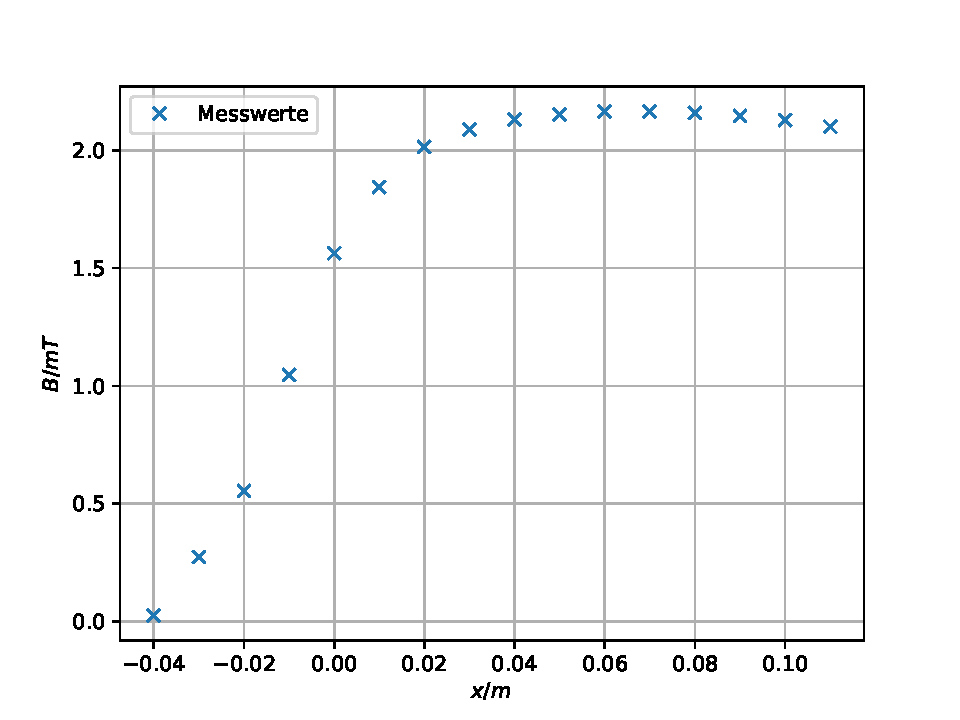
\includegraphics[width=\textwidth]{Langesp.pdf}
  \caption{B-Feld der langen Spule}
  \label{fig:ls}
\end{figure}
Als experimenteller Vergleichswert wird der Messwert gewählt, der sich in der Mitte der Spule befindet:
\begin{equation*}
  B_{LS, e} = \SI{2.160e-3}{T}
\end{equation*}
\\abgelesen.
\\Der theoretische Wert des Magnetfelds in der Spule wird mit Formel \eqref{eqn:ls} errechnet.
Es ergibt sich
\begin{equation*}
  B_{LS, t} = \SI{2.094395e-3}{T}.
\end{equation*}
\FloatBarrier

\subsubsection{Kurze Spule}
Die Ergebnisse der Vermessung der kurzen Spule sind in der Tabelle \ref{tab:ks} zu sehen.
Die Messwerte sind wiederum in der Abbildung \ref{fig:ks} aufgetragen.
Der Anfangspunkt der Spule liegt im Ursprung, die Mitte der Spule bei $x=\SI{0.04}{m}$.

\begin{table}
  \centering
  \caption{Messdaten zur kurzen Spule}
  \label{tab:ks}
  \begin{tabular}{c c c c}
    \toprule
     x/m &	 B/$\SI{e-3}{T}$	 \\
    \midrule
    -0,03	& 0,066\\
    -0,02	& 0,211\\
    -0,01	& 0,451\\
     0,00	& 0,900\\
     0,01	& 1,471\\
     0,02	& 1,782\\
     0,03	& 1,885\\
     0,04	& 1,779\\
     0,05	& 1,507\\
     0,06	& 1,105\\
     0,07	& 0,556\\
     0,08	& 0,254\\
     0,09	& 0,105\\
     0,10	& 0,035\\
    \bottomrule
  \end{tabular}
\end{table}

\begin{figure}[h!]
  \centering
  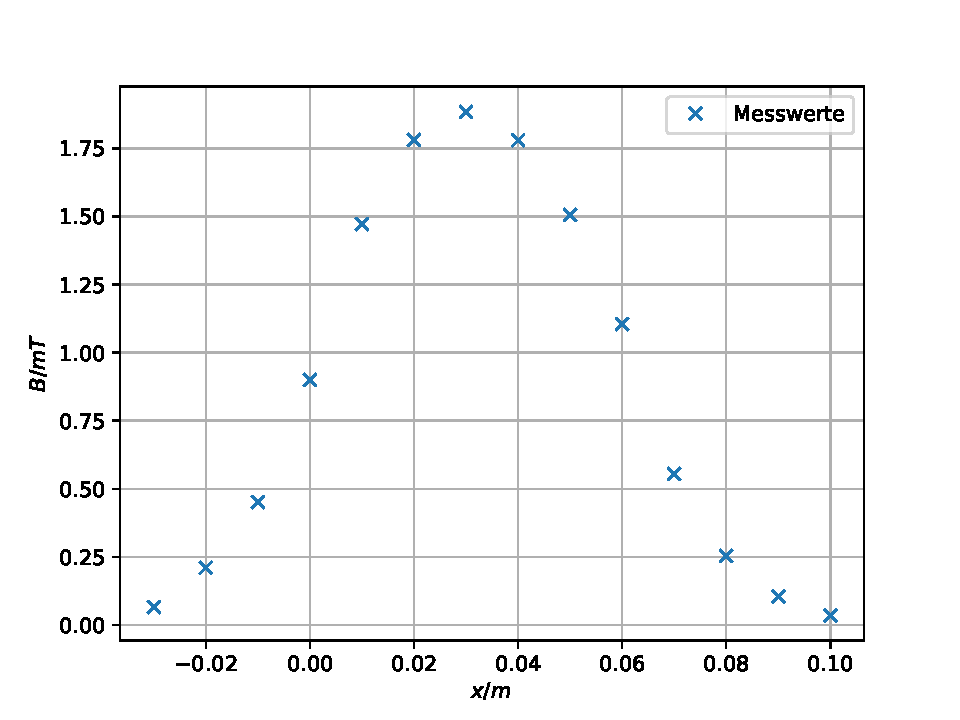
\includegraphics[width=\textwidth]{Kurzesp.pdf}
  \caption{B-Feld der kurzen Spule}
  \label{fig:ks}
\end{figure}
Als experimenteller Wert wird das Maximum der magnetischen Flussdichte
\begin{equation*}
  B_{KS, e} = \SI{1.885e-3}{T}
\end{equation*}
\\gewählt.
\\Mit Formel \eqref{eqn:ls} wird ein Theoriewert angenähert.
Es ergibt sich
\begin{equation*}
  B_{KS, t} = \SI{4.712389e-3}{T}.
\end{equation*}
\FloatBarrier

\subsection{Magnetfelder einer Helmholtzspule}
Das Magnetfeld einer Helmholtzspule wird für die Spulenabstände $d_{1}=\SI{0.08}{m}$, $d_{2}=\SI{0.10}{m}$ und $d_{3}=\SI{0.12}{m}$ gemessen.
Die Messwerte sind in Tabelle \ref{tab:h8}, Tabelle \ref{tab:h10} und Tabelle \ref{tab:h12} aufgeführt.
Die Messwerte sind in Abbildung \ref{fig:h8}, Abbildung \ref{fig:h10} und Abbildung \ref{fig:h12} aufgetragen.

\documentclass[captions=tableheading]{scrartcl}
\usepackage{booktabs}
\usepackage{pdflscape}




\begin{document}
%\begin{landscape}


\begin{table}
  \centering
  \caption{Messdaten}
  \label{tab:some_data}
  \begin{tabular}{c c }
    \toprule
     x &	 B	   \\
     cm &   mT  \\
    \midrule
      \documentclass[captions=tableheading]{scrartcl}
\usepackage{booktabs}
\usepackage{pdflscape}




\begin{document}
%\begin{landscape}


\begin{table}
  \centering
  \caption{Messdaten}
  \label{tab:some_data}
  \begin{tabular}{c c }
    \toprule
     x &	 B	   \\
     cm &   mT  \\
    \midrule
      \documentclass[captions=tableheading]{scrartcl}
\usepackage{booktabs}
\usepackage{pdflscape}




\begin{document}
%\begin{landscape}


\begin{table}
  \centering
  \caption{Messdaten}
  \label{tab:some_data}
  \begin{tabular}{c c }
    \toprule
     x &	 B	   \\
     cm &   mT  \\
    \midrule
      \input{Helm8.txt}
    \bottomrule
  \end{tabular}
\end{table}

%\end{landscape}
\end{document}

    \bottomrule
  \end{tabular}
\end{table}

%\end{landscape}
\end{document}

    \bottomrule
  \end{tabular}
\end{table}

%\end{landscape}
\end{document}

\begin{figure}[h!]
  \centering
  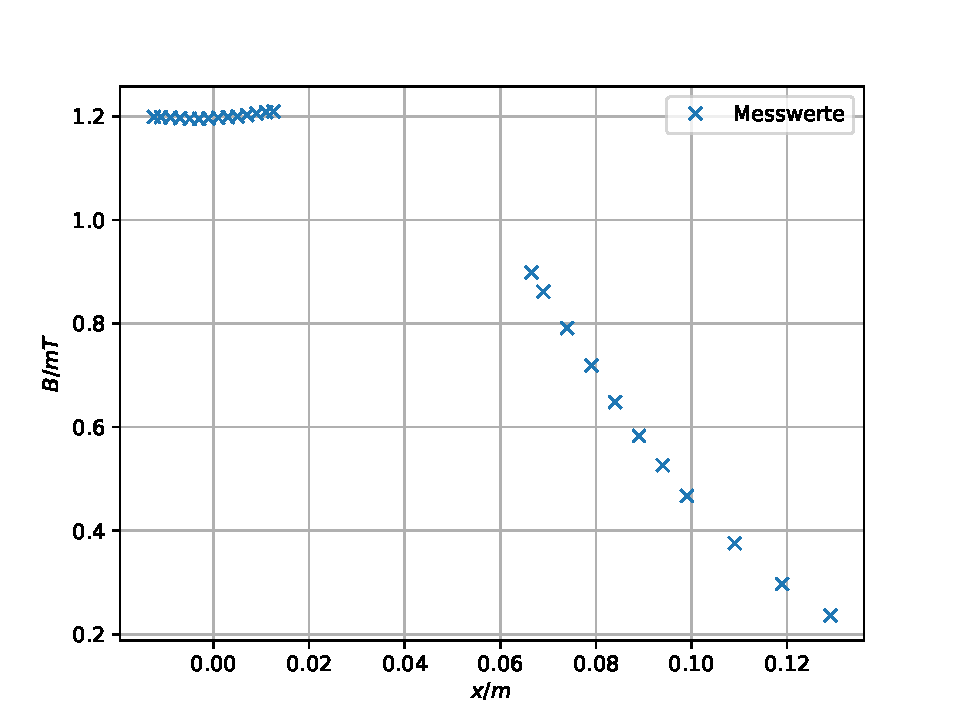
\includegraphics[width=\textwidth]{Helm8.pdf}
  \caption{B-Feld der Helmholzspule mit $d_{1}=\SI{0.08}{m}$}
  \label{fig:h8}
\end{figure}

\documentclass[captions=tableheading]{scrartcl}
\usepackage{booktabs}
\usepackage{pdflscape}




\begin{document}
%\begin{landscape}


\begin{table}
  \centering
  \caption{Messdaten}
  \label{tab:some_data}
  \begin{tabular}{c c }
    \toprule
     x &	 B	   \\
     cm &   mT  \\
    \midrule
      \documentclass[captions=tableheading]{scrartcl}
\usepackage{booktabs}
\usepackage{pdflscape}




\begin{document}
%\begin{landscape}


\begin{table}
  \centering
  \caption{Messdaten}
  \label{tab:some_data}
  \begin{tabular}{c c }
    \toprule
     x &	 B	   \\
     cm &   mT  \\
    \midrule
      \documentclass[captions=tableheading]{scrartcl}
\usepackage{booktabs}
\usepackage{pdflscape}




\begin{document}
%\begin{landscape}


\begin{table}
  \centering
  \caption{Messdaten}
  \label{tab:some_data}
  \begin{tabular}{c c }
    \toprule
     x &	 B	   \\
     cm &   mT  \\
    \midrule
      \input{Helm10.txt}
    \bottomrule
  \end{tabular}
\end{table}

%\end{landscape}
\end{document}

    \bottomrule
  \end{tabular}
\end{table}

%\end{landscape}
\end{document}

    \bottomrule
  \end{tabular}
\end{table}

%\end{landscape}
\end{document}

\begin{figure}[h!]
  \centering
  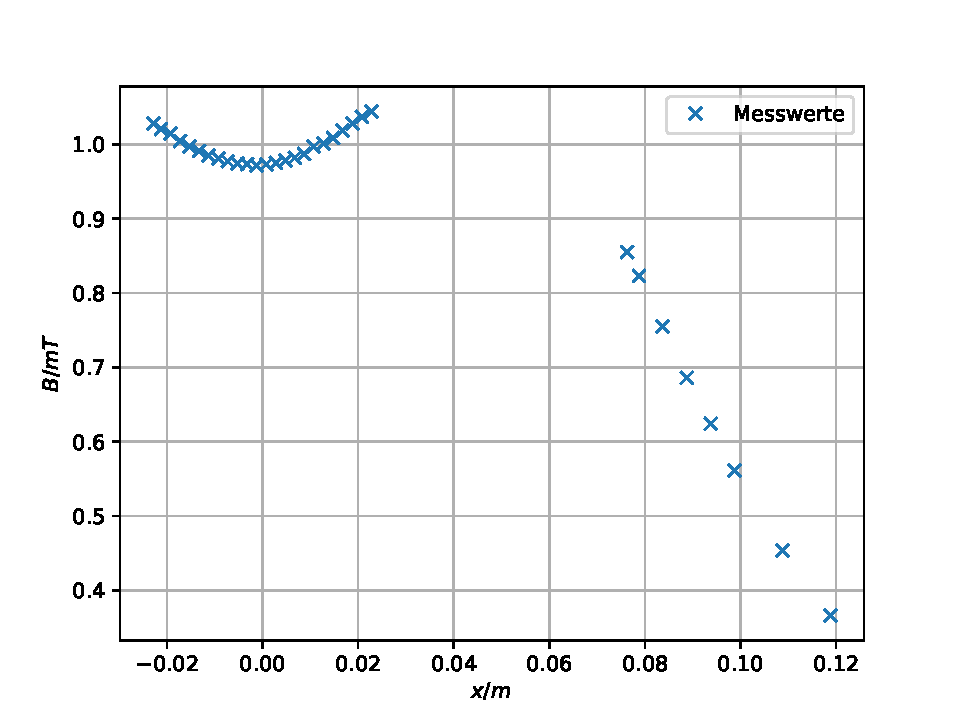
\includegraphics[width=\textwidth]{Helm10.pdf}
  \caption{B-Feld der Helmholzspule mit $d_{2}=\SI{0.10}{m}$}
  \label{fig:h10}
\end{figure}


\begin{table}[h!]
  \centering
  \caption{Messdaten zur Helmholzspule mit $d_{3}=\SI{0.12}{m}$}
  \label{tab:h12}
  \begin{tabular}{c c c c}
    \toprule
     x/m &	 B/$\SI{e-3}{T}$  &  x/m &	 B/$\SI{e-3}{T}$ \\
    \midrule
    -0,03275	& 0,915 &      0,01075	& 0,799\\
    -0,03125	& 0,906 &      0,01275	& 0,808\\
    -0,02925	& 0,892 &      0,01475	& 0,817\\
    -0,02725	& 0,879 &      0,01675	& 0,829\\
    -0,02525	& 0,866 &      0,01875	& 0,839\\
    -0,02325	& 0,852 &      0,02075	& 0,854\\
    -0,02125	& 0,842 &      0,02275	& 0,866\\
    -0,01925	& 0,831 &      0,02475	& 0,879\\
    -0,01725	& 0,818 &      0,02675	& 0,893\\
    -0,01525	& 0,809 &      0,02875	& 0,909\\
    -0,01325	& 0,800 &      0,03075	& 0,922\\
    -0,01125	& 0,794 &      0,03275	& 0,937\\
    -0,00925	& 0,788 &      0,08675  & 0,825\\
    -0,00725	& 0,782 &      0,08875  & 0,801\\
    -0,00525	& 0,780 &      0,09375  & 0,735\\
    -0,00325	& 0,777 &      0,09875  & 0,665\\
    -0,00125	& 0,776 &      0,10375	& 0,610\\
     0,00075	& 0,776 &      0,10875	& 0,543\\
     0,00275	& 0,778 &      0,11875	& 0,437\\
     0,00475	& 0,781 &      0,12875	& 0,345\\
     0,00675	& 0,786 &      0,13875	& 0,273\\
     0,00875	& 0,792 &          -    &   -  \\

    \bottomrule
  \end{tabular}
\end{table}

\begin{figure}[h!]
  \centering
  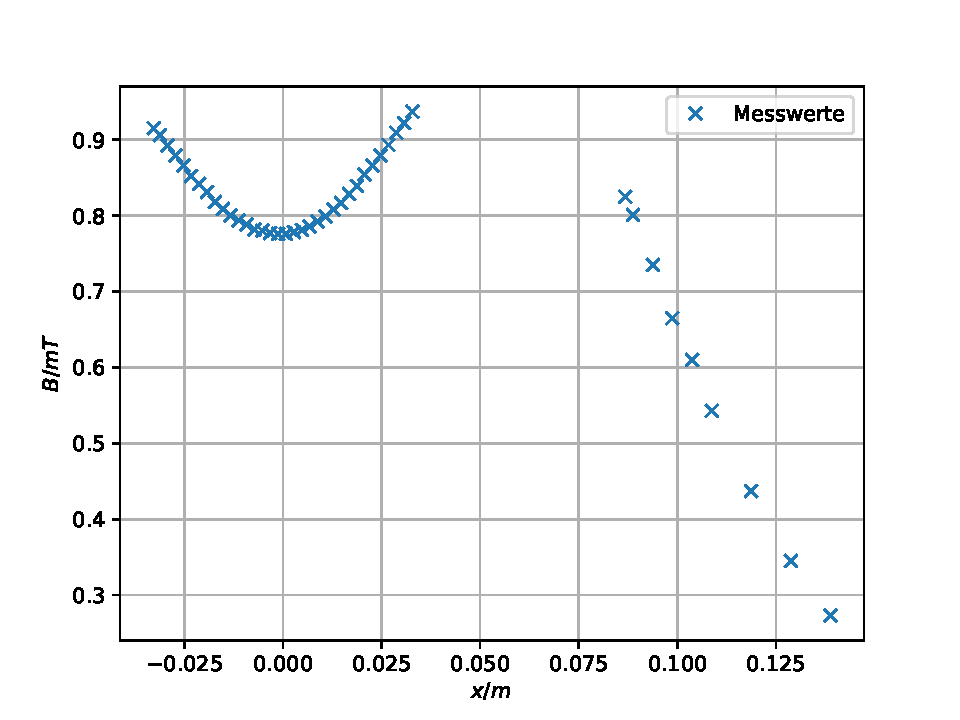
\includegraphics[width=\textwidth]{Helm12.pdf}
  \caption{B-Feld der Helmholzspule mit $d_{3}=\SI{0.12}{m}$}
  \label{fig:h12}
\end{figure}

Folgende Werte werden als magnetische Flussdichte in der Mitte der beiden Spulen gemessen.
\\Für den Spulenabstand $d_{1}=\SI{0.08}{m}$:
\begin{equation*}
  B_{H1, e} = \SI{11.97e-4}{T}.
\end{equation*}
\\Für den Spulenabstand $d_{2}=\SI{0.10}{m}$:
\begin{equation*}
  B_{H2, e} = \SI{9.73e-4}{T}.
\end{equation*}
\\Für den Spulenabstand $d_{3}=\SI{0.12}{m}$:
\begin{equation*}
  B_{H3, e} = \SI{7.76e-4}{T}.
\end{equation*}
\\Die theoretischen Werte werden mit Formel \eqref{eqn:helm} ermittelt.
Es ergeben sich die folgenden Werte:
\begin{equation*}
  B_{H1, t} = \SI{12.01395e-4}{T}
\end{equation*}
\begin{equation*}
  B_{H2, t} = \SI{9.573353e-4}{T}
\end{equation*}
\begin{equation*}
  B_{H3, t} = \SI{7.548060e-4}{T}
\end{equation*}
\FloatBarrier


\subsection{Hysteresekurve}
Die Messwerte für die Hysteresekurve sind in der Tabelle \ref{tab:hys} zu sehen.
In der Abbildung \ref{fig:hyst} sind die Messwerte aufgetragen.
Aus der Graphik lassen sich die äquvalenten Werte für die Remanenz und die Koerzitivkraft ablesen.
Das Äquvalent der Remanenz hat den Wert
\begin{equation*}
  B_r = \SI{-123.2}{mT}.
\end{equation*}
\\Das Äquvalent der Koerzitivkraft lässt sich als
\begin{equation*}
  H_c = \SI{-0,7}{A}
\end{equation*}
bestimmen.
\documentclass[captions=tableheading]{scrartcl}
\usepackage{booktabs}
\usepackage{pdflscape}




\begin{document}
%\begin{landscape}


\begin{table}
  \centering
  \caption{Messdaten}
  \label{tab:some_data}
  \begin{tabular}{c c c c c c c c }
    \toprule
     I &	 B	 & & I &  B  & & I & B  \\
     A &   mT  & & A & mT  & & A & mT \\
    \midrule
      \documentclass[captions=tableheading]{scrartcl}
\usepackage{booktabs}
\usepackage{pdflscape}




\begin{document}
%\begin{landscape}


\begin{table}
  \centering
  \caption{Messdaten}
  \label{tab:some_data}
  \begin{tabular}{c c c c c c c c }
    \toprule
     I &	 B	 & & I &  B  & & I & B  \\
     A &   mT  & & A & mT  & & A & mT \\
    \midrule
      \documentclass[captions=tableheading]{scrartcl}
\usepackage{booktabs}
\usepackage{pdflscape}




\begin{document}
%\begin{landscape}


\begin{table}
  \centering
  \caption{Messdaten}
  \label{tab:some_data}
  \begin{tabular}{c c c c c c c c }
    \toprule
     I &	 B	 & & I &  B  & & I & B  \\
     A &   mT  & & A & mT  & & A & mT \\
    \midrule
      \input{tabneu.txt}
    \bottomrule
  \end{tabular}
\end{table}

%\end{landscape}
\end{document}

    \bottomrule
  \end{tabular}
\end{table}

%\end{landscape}
\end{document}

    \bottomrule
  \end{tabular}
\end{table}

%\end{landscape}
\end{document}

\begin{figure}[h!]
  \centering
  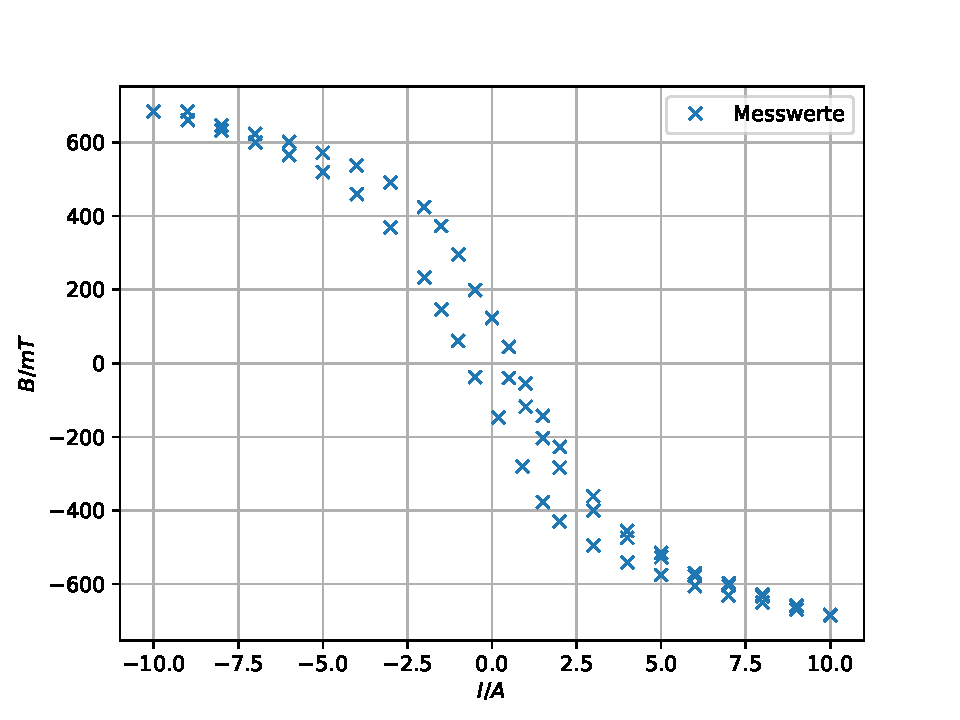
\includegraphics[width=\textwidth]{hysterese.pdf}
  \caption{Hysteresekurve}
  \label{fig:hyst}
\end{figure}
\FloatBarrier
